\documentclass[a4paper,14pt]{extarticle}
\usepackage[T2A]{fontenc}
\usepackage[utf8]{inputenc}
\usepackage[english,russian]{babel}
\usepackage{amsmath,amsfonts,amsthm, mathtools}
\usepackage{amssymb}
\usepackage{icomma}
\usepackage{graphicx}
\usepackage{wrapfig}
\RequirePackage{longtable}
\usepackage{soulutf8} 
\usepackage{geometry}
\geometry{top=20mm}
\geometry{bottom=20mm}
\geometry{left=20mm}
\geometry{right=20mm}
% новая команда \RNumb для вывода римских цифр
\newcommand{\RNumb}[1]{\uppercase\expandafter{\romannumeral #1\relax}}

\usepackage{cmap}					
\usepackage{mathtext} 				
			
		

\usepackage{multirow}
\usepackage{graphicx}
\usepackage{wrapfig}
\usepackage{tabularx}
\usepackage{float}
\usepackage{hyperref}
\hypersetup{colorlinks=true,urlcolor=blue}
\usepackage[rgb]{xcolor}
\usepackage{amsmath,amsfonts,amssymb,amsthm,mathtools} 
\usepackage{icomma} 
\usepackage{euscript}
\usepackage{mathrsfs}
\usepackage{enumerate}
\usepackage{caption}
\usepackage{enumerate}
\mathtoolsset{showonlyrefs=true}

\usepackage{caption}
\usepackage{subcaption}

\usepackage[europeanresistors, americaninductors]{circuitikz}
\DeclareMathOperator{\sgn}{\mathop{sgn}}
\newcommand*{\hm}[1]{#1\nobreak\discretionary{}
	{\hbox{$\mathsurround=0pt #1$}}{}}

\begin{document}
	\begin{center}
		\textit{Федеральное государственное автономное образовательное\\ учреждение высшего образования }
		
		\vspace{0.5ex}
		
		\textbf{«Московский физико-технический институт\\ (национальный исследовательский университет)»}
	\end{center}
	
	\vspace{10ex}
	
	
	\begin{center}
		\vspace{13ex}
		
		\textbf{Лабораторная работа №1.1.4}
		
		\vspace{1ex}
		
		по курсу общей физики
		
		на тему:
		
		\textbf{\textit{<<Измерение интенсивности радиационного фона>>}}
		
		\vspace{30ex}
		
		\begin{flushright}
			\noindent
			\textit{Работу выполнил:}\\  
			\textit{Третьяков Александр \\(группа Б02-206)}
		\end{flushright}
		\vfill
		Долгопрудный \\ \today
		
		%\setcounter{page}{1}
	\end{center}
	\newpage	
	
	
	
	• Цель работы: применение методов обработки экспериментальных данных для изучения статистических закономерностей при измерении интесивности радиационного фона
	
	
	В работе исппользуется: счетчик  Гейгера-Мюллера(СТС-6), блок питания, компьютер с интерфейсом связи со счетчиком.
	\newline
	
	• Теоретические сведения:
	\newline
	
	Значительную часть радиационного фона составляет поток космических частиц, изменяющийся со временем случайным образом.
	Космические лучи разделяют на первичные - поток стабилных частиц, имеющих большую кинетическую энергию ($10^{9} - 10^{21}$ эВ) и вторичные, которые возникают при взаимодействии первичных с атмосферой Земли и составляют основную часть космичексих лучей, доходящих до поверхности Земли.
	Установлено, что в космическом пространстве поток частиц изотропен.
	\newline
	
	
	• Устройство счетчика Гейгера-Мюллера.
	\newline
	
	Счетчик, используемый в данной работе (СТС-6), представляет собой  наполненный газом сосуд с двумя электродами:
	катодом(тонкостенным металлическим цилиндром) и анодом(тонкой нитью, натянутой вдоль оси циллиндра).
	На электроды подается напряжение 400 В.
	Частицы космических лучей ионизируют газ, находящийся в счетчике, а также выбивают электроны из его стенок; таким образом появляются свободные электроны. Под действием электрического поля между электродами электрон разгоняется и врезается в другие атомы, вибивая из них новые электроны.Развиваясь лавинообразно, этот процесс завершается образованием в межэлектродном пространстве электронно-ионного облака, резко увеличивающего его проводимость. По
	существу, при попадании в счетчик Гейгера частицы в нём вспыхивает (зажигается) самостоятельный
	газовый разряд, видимый (если баллон прозрачный) даже простым глазом.
	\newline
	
	
	
	
	• Основные расчётные формулы:
	\newline
	
	Ошибка единичного измерения $\sigma = \sqrt{n}$. (В данном эксперименте n - это число импульсов)
	
	В полосе $n\pm\sqrt{n}$ лежит 68\% точек.
	
	Ошибка среднего $\overline{\sigma} = \sqrt{\overline{n}}$.
	
	Стандартное отклонение $\sigma = \dfrac{\overline{\sigma}}{\sqrt{N}}$, где N - это количество измерений.
	\newline
	

	\newpage
	• Графики:
	\newline
	
	\begin{wrapfigure}[10]{1}{0.6\linewidth}
		
\includegraphics[width=\linewidth ]{1}
		\caption{Основной эксперимент}
	\end{wrapfigure}

По этому графику через равные промежутки времени измеряем полосу, в которую попадают все точки, и  укорачиваем ее в $\frac{2}{3}$ раза, а потом делим пополам. Это и будет наша ошибка. Также по графику можем оценить среднее значение и сравнить его с реальным с помощью графика ниже.
\newline
	\bigskip
	\\
	\\
	\\
	\\
	\\
		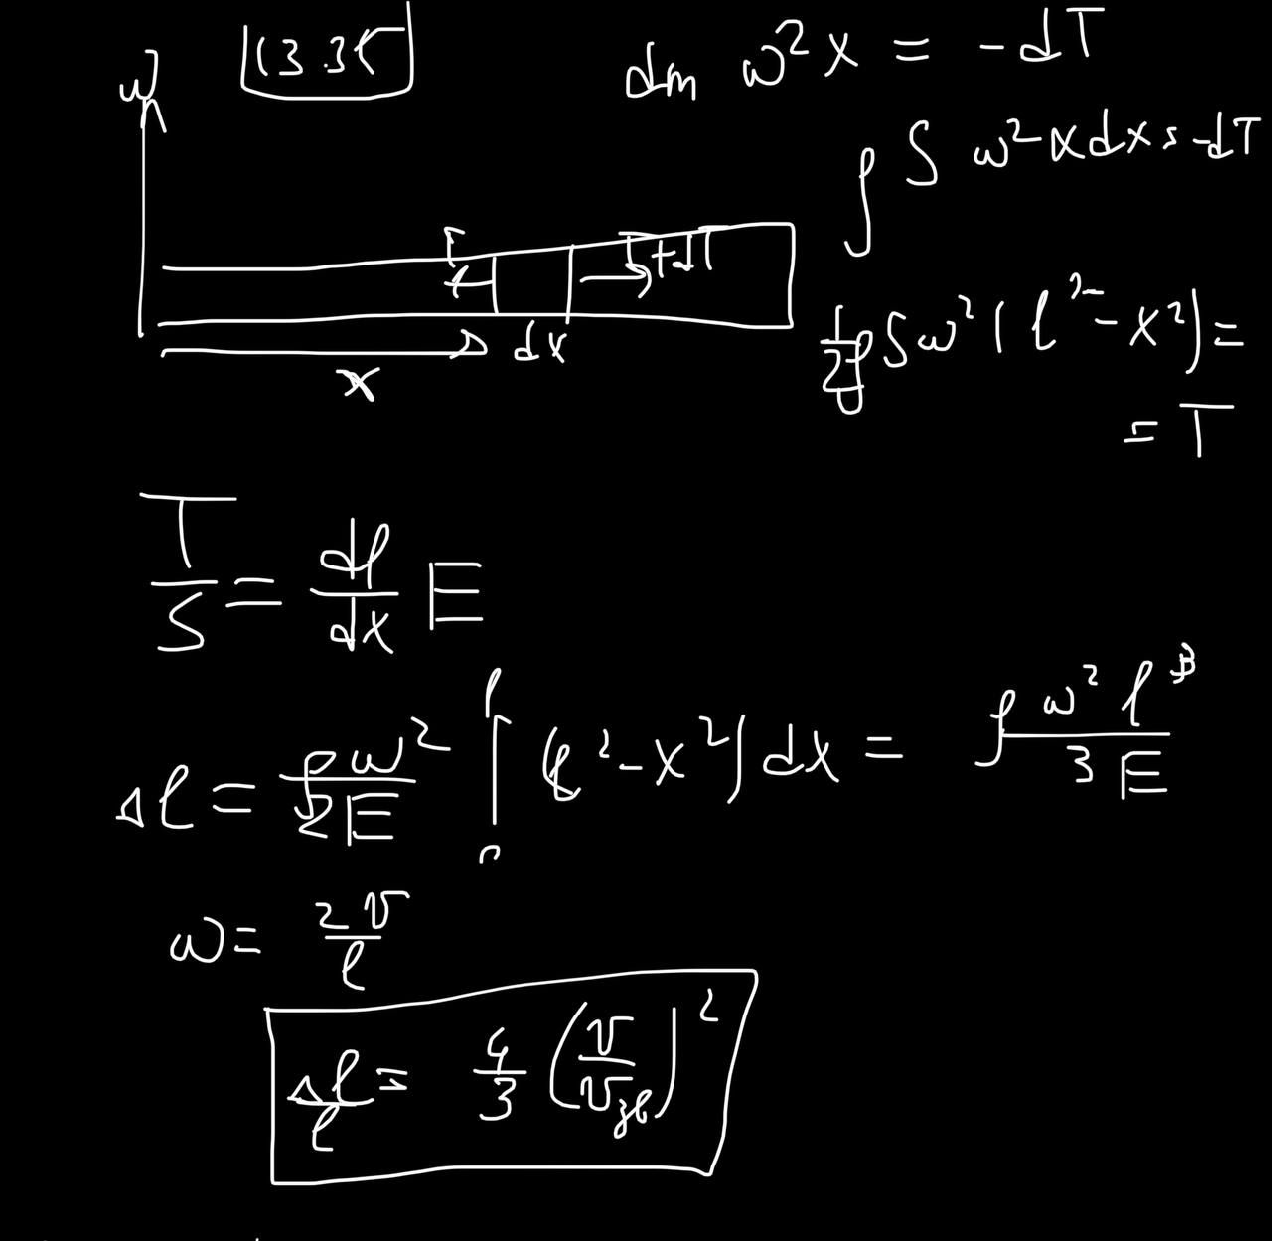
\includegraphics[width=\linewidth * 2]{2}
	
	
	
	\newpage
	\begin{wrapfigure}[19]{1}{0.6\linewidth}
		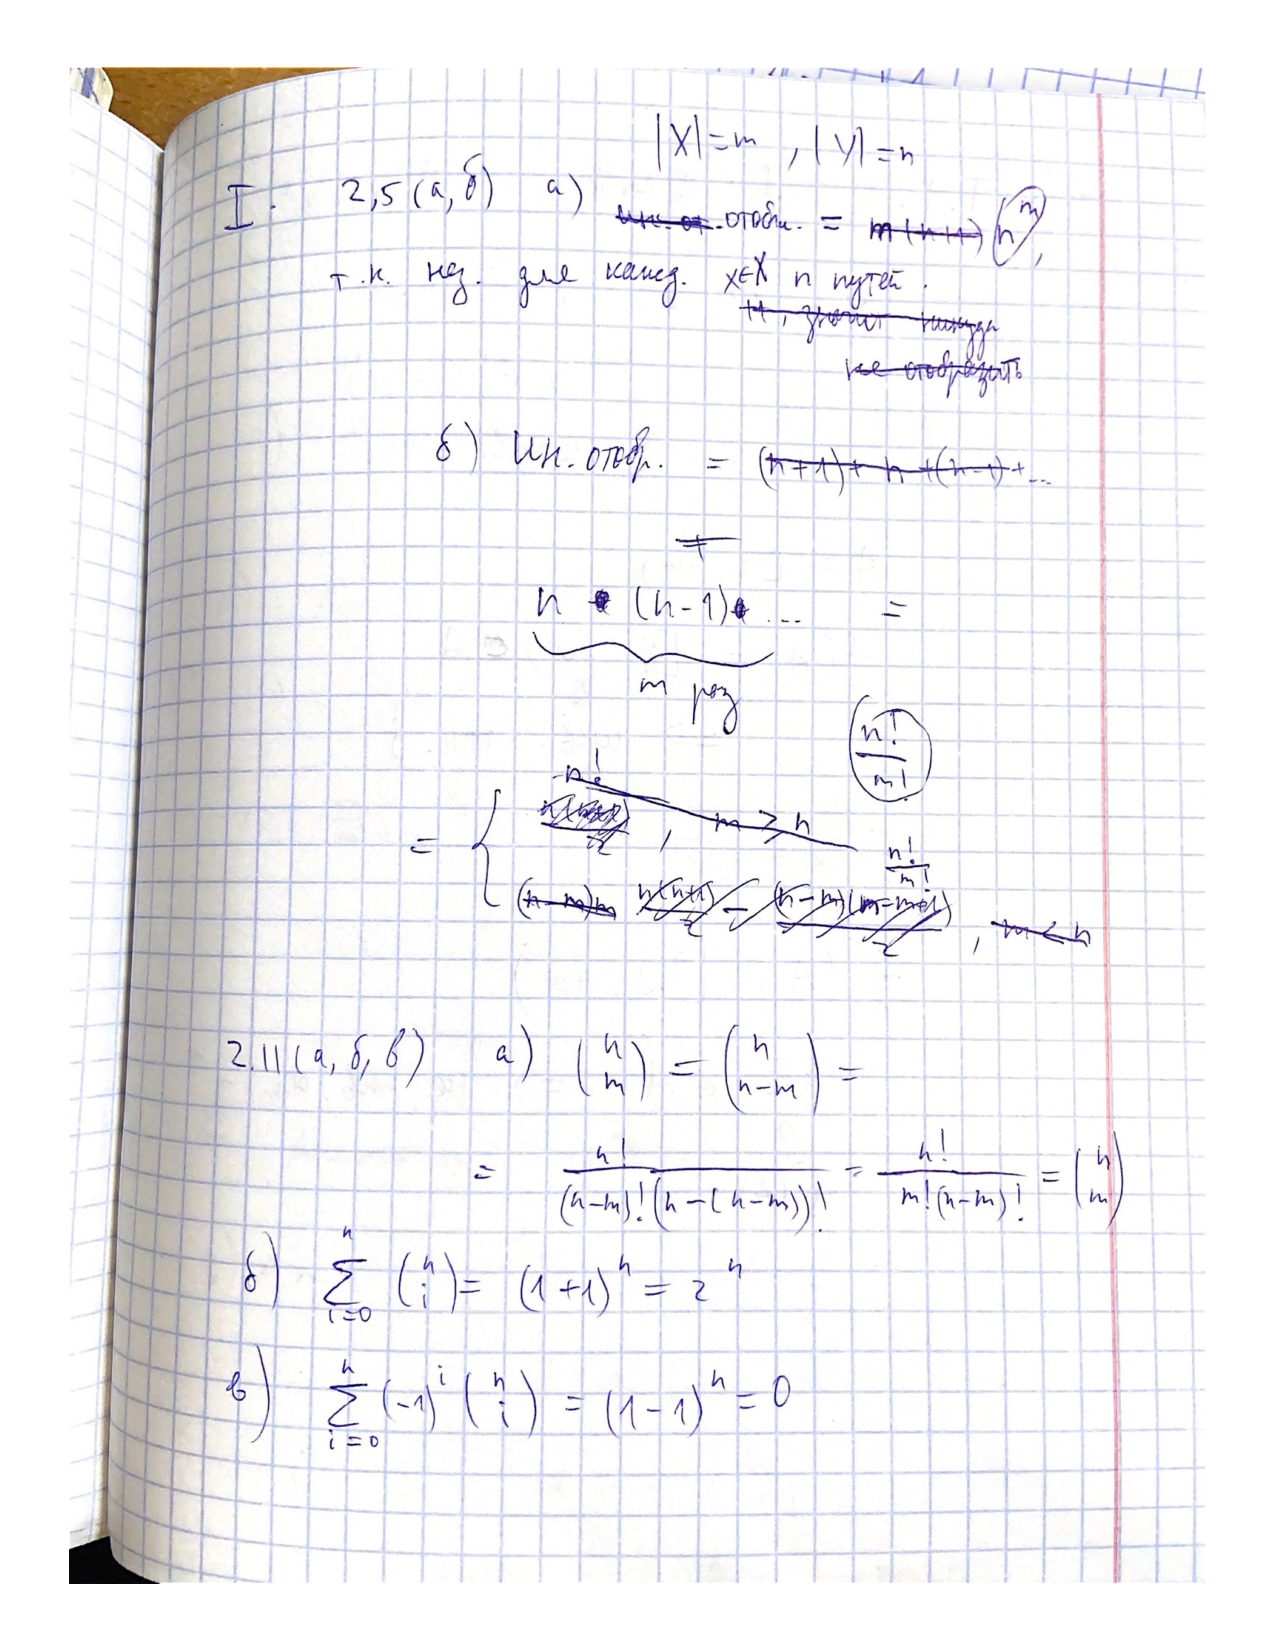
\includegraphics[width=\linewidth ]{3}
		\caption{Стандартное отклонение}
	


	\includegraphics[width=\linewidth ]{4}
	\caption{Гистограмма}
\end{wrapfigure}
Опираясь на предыдущие данные, которые мы уже получили(ошибку среднего), вычисляем стандартное отклонение по формуле $\sigma = \dfrac{\overline{\sigma}}{\sqrt{N}}$ и сравниваем с реальным по графику.
\newline
\bigskip
\\
\\
\\
\\
\\
По гистограмме видим на какое число импульсов приходится максимум и убеждаемся в нормальности распределения нашей случайной величины, так как кривая красиво ложится на гауссиану.
\newline
\bigskip
\\
\\
\\
\\
\\
\\
\\
\includegraphics[width=10cm ]{5}
\includegraphics[width=8cm ]{6}
Сравнив результаты основного и демонстрационного опыта, можно заметить, что данные получились довольно похожими, даже несмотря на меньшее количество измерений во втором опыте. Из этого можно сделать вывод, что распределение нормальное, а ошибка случайная.
\newpage
 
	• Результаты измерений и обработка данных:
	
	
		\begin{center}
		
			\begin{tabular}{|c|c|c|c|c|c|}
			\hline
				Количество измерений & 80 & 160 & 240 & 320 & 400  \\ \hline
				Оценка ошибки по полосе & 2.0 & 2.5 & 2.5 & 3.0 & 3.2   \\ \hline
				Оценка среднего & 12 & 12 & 12 & 12 & 12   \\ \hline
			    Реальное среднее & 11.9 & 11.3 & 11.2 & 11.5 & 11.4   \\  \hline
				Оценка ошибки среднего & 3.5 & 3.5 & 3.5 & 3.5 & 3.5  \\ \hline
				Оценка стандартного отклонения & 0.39 & 0.28 & 0.22 & 0.20 & 0.18  \\  \hline
				Реальное стандартное отклонение & 0.39 & 0.23 & 0.21 & 0.19 & 0.18   \\ \hline
			
			\end{tabular}
		\includegraphics[width=14cm ]{7}
		\includegraphics[width=8cm ]{graph1}
		\includegraphics[width=8cm ]{graph2}
		Слева предствалена гистограмма, где данные за каждые 10 секунд, а справа за каждые 20. По гистограммам можно понять, что наибольшее число случаев приходится на значение примерно 10 импульсов за 10 секунд.
		\end{center}
		%\caption{Заголовок мог быть и здесь}
	

	
	
	• Заключение:
	\newline
	
Нам удалось измерить интенсивность радиационного фона. Мы применили статистические методы для анализа данных и пришли к выводу, что радиационный фон стабилен. Также нам удалось довольно хорошо оценить погрешности, среднее значение и стандартное отклонение.
\end{document}